\documentclass[12pt,reqno]{amsart}
\usepackage[margin=3cm]{geometry}

\usepackage{amsmath, amssymb, amsfonts, tikz,enumerate, graphicx, textcomp, caption, wrapfig, amsthm, todonotes, verbatim, cleveref, caption, float, mathabx, url}
\usetikzlibrary{calc, arrows}
\usepackage[procnames]{listings}
\usepackage{color, subfig}
\usepackage[section]{placeins}

\usepackage{color}
\definecolor{purple}{rgb}{0.5,0,1}

\newenvironment{dami}{
  \medskip
\begin{color}{blue}
    \textcolor{purple}{\textbf{Dami:}} 
}{
\end{color}
  \medskip
}


\newenvironment{cat}{
  \medskip
\begin{color}{red}
    \textcolor{red}{\textbf{Catherine:}} 
}{
\end{color}
  \medskip
}

\definecolor{keywords}{RGB}{255,0,90}
\definecolor{comments}{RGB}{0,0,113}
\definecolor{red}{RGB}{160,0,0}
\definecolor{green}{RGB}{0,150,0}
\lstdefinelanguage{Magma}%
  {%
   otherkeywords={:=,+:=,-:=,*:=},%
          % functions
   procnamekeys={function,func,intrinsic,procedure,proc},%
         % Booleans
   morekeywords={true,false},%
          % relations
   morekeywords=[2]{adj,and,cat,cmpeq,cmpne,diff,div,eq,ge,gt,in,is,join,le,lt,%
          meet,mod,ne,notadj,notin,notsubset,or,sdiff,subset,xor},%
          % keywords
   morekeywords=[3]{assigned,break,by,case,catch,continue,declare,default,%
          delete,do,elif,else,end,eval,exists,exit,for,forall,fprintf,if,local,%
          not,print,printf,quit,random,read,readi,repeat,restore,save,select,%
          then,time,to,try,until,vprint,vprintf,vtime,when,where,while},%
          % directives
   morekeywords=[4]{clear,forward,freeze,iload,import,load},%
          % error checks
   morekeywords=[5]{assert,assert2,assert3,error,require,requirege,requirerange},%
          % constructors
   morekeywords=[6]{car,comp,cop,elt,ext,frac,hom,ideal,iso,lideal,loc,map,%
          ncl,pmap,quo,rec,recformat,rep,rideal,sub},%
          % other constructors (semi-reserved)
   morekeywords=[7]{AbelianGroup,AdditiveCode,AffineAlgebra,Algebra,%
          AssociativeAlgebra,Character,CliffordAlgebra,Design,Digraph,%
          ExtensionField,FPAlgebra,FiniteAffinePlane,FiniteProjectivePlane,%
          Graph,Group,GroupAlgebra,IncidenceStructure,LieAlgebra,LinearCode,%
          LinearSpace,MatrixAlgebra,MatrixGroup,MatrixRing,Monoid,%
          MultiDigraph,MultiGraph,NearLinearSpace,Network,PartialMap,%
          PermutationGroup,PolycyclicGroup,QuaternionAlgebra,Semigroup,%
          ZModule},%
          % functions
   morekeywords={[8]function,func,intrinsic,procedure,proc,return},%
      sensitive,%
      morecomment=[l]//,%
      morecomment=[s]{/*}{*/},%
      morecomment=[s]{\{}{\}},%
      morestring=[b]"%
  }[keywords,procnames,comments,strings]%
\lstset{language=Python, 
        basicstyle=\ttfamily\small, 
        keywordstyle=\color{keywords},
        commentstyle=\color{comments},
        stringstyle=\color{red},
        breaklines=true,
        showstringspaces=false,
        identifierstyle=\color{green},
        procnamekeys={def,class}}
%\usepackage[T1]{fontenc}
%\usepackage[urw-garamond]{mathdesign}
\usepackage{tikz-cd}\tikzset{node distance=2cm, auto}
\DeclareMathOperator{\Aut}{Aut}
\DeclareMathOperator{\Hom}{Hom}
\DeclareMathOperator{\Jac}{Jac}
\DeclareMathOperator{\Sym}{Sym}
\DeclareMathOperator{\Alt}{Alt}
\DeclareMathOperator{\Corr}{Corr}
\DeclareMathOperator{\im}{im}
\DeclareMathOperator{\uncurry}{uncurry}
\DeclareMathOperator{\Pic}{Pic}
\DeclareMathOperator{\Div}{Div}
\newcommand{\C}{\mathbb{C}}
\newcommand{\Z}{\mathbb{Z}}
\newcommand{\F}{\mathbb{F}}
\newcommand{\G}{\mathbb{G}}
\newcommand{\Q}{\mathbb{Q}}
\newcommand{\R}{\mathbb{R}}
\newcommand{\n}{\newline}
\newcommand{\mc}{\mathcal}
\newcommand{\te}{\text}
\newcommand{\bb}{\mathbb}
\renewcommand{\P}{\mathbb{P}}
\newcommand{\BBF}{\overline{\F_p}}
\newcommand\mapsfrom{\mathrel{\reflectbox{\ensuremath{\mapsto}}}}
\definecolor{codegray}{gray}{0.9}
\newcommand{\code}[1]{\colorbox{codegray}{\texttt{#1}}}
\newtheorem{theorem}{Theorem}
\newtheorem*{thm*}{Theorem}
\newtheorem*{proposition}{Proposition}
\newtheorem{lemma}[theorem]{Lemma}
\newtheorem*{lemma*}{Lemma}
\newtheorem*{qlemma*}{``Lemma"}
\newtheorem{cor}[theorem]{Corollary}
\newtheorem{conjecture}[theorem]{Conjecture}
\newtheorem{postulate}[theorem]{Postulate}
\newtheorem*{question}{Question}
\theoremstyle{definition}
\newtheorem{defn}{Definition}
\newtheorem{example}[theorem]{Example}
\theoremstyle{remark}
\newtheorem*{remark}{Remark}
\newtheorem*{notation}{Notation}
\newtheorem*{note}{Note}
\newcommand{\sss}{\ss$\text{ }$}
\newcommand{\ti}{\todo[inline]}
\newcommand{\DD}{\Delta\kern -8.3pt {\diamond} \kern -4.5pt \cdot \:}
\newenvironment{myproof}[1][``\proofname '']{%
  \proof[ #1]%
}{\endproof}




\title{Computing Automorphism Groups via Constructing Tessellations} 
\author{Dami Lee and Catherine Ray}

\begin{document}

	
\maketitle

%In this paper, we calculate and interpret the interaction between the automorphism group of a Riemann surface and the automorphism group of its Jacobian. We exposit and expand some calculational techniques from computational arithmetic geometry and hyperbolic geometry. We calculate the automorphism groups of some well-known surfaces such as Klein's quartic, Fermat's quartic, and Bring's curve. For further examples, we exploit the fact that the previously mentioned surfaces can be described as cyclically branched coverings over punctured spheres. We also discuss the modular curve $X_0(63),$ which is not a cyclic cover over a sphere. We find several principal polarizations on many Jacobians of these Riemann surfaces, and the automorphism groups with respect to each of these polarizations. We discuss and answer questions on Jacobians with multiple principal polarizations. 


\begin{abstract}
Given a symmetric surface, we introduce a new conjectural method for computing its automorphism group by constructing and counting a particular tessellation of the surface. More specifically, we consider any cyclically branched surface with either equal or unequal weight Weierstrass points, and construct a regular hyperbolic tessellation on this surface which is preserved under the automorphism group. Examples we explore include Klein's quartic, Fermat's quartic, and Bring's curve. We verify this conjecture up to genus 5 with programs based on the algorithms of Bruin-Sijsling-Zotine.
\end{abstract}

\section{Introduction}

In \cite{dami}, the first author develops a method to compute the automorphism group of Fermat's quartic by constructing a particular tesselation. This method works particularly well on highly symmetric surfaces, e.g. those whose Weierstrass points have uniform weight. 

Lee presents Fermat's quartic as an eightfold cyclically branched cover over a thrice punctured sphere and finds a regular hyperbolic tessellation on the surface that is preserved under the automorphism group. Using this ``all-seeing" tessellation, Lee computes the automorphism group of Fermat's quartic in a generator-relation format. Lee's method (all-seeing method?) provides a different way to present automorphisms of a curve concretely, without presenting the automorphism group as an action on the coefficients of a polynomial describing the curve (as is done in Silverman, appendix A). 

This project began from the second author wondering if the first authors method for computing the automorphism group of Fermat's quartic could be applied in more generality, to model the automorphism group of the principally-polarized Jacobian of a curve (where curve here means cyclically branched cover of the punctured sphere). The aim was to embed the all-seeing tessellation from the original curve $C$ into the Jacobian, and extend it to a tesselation on the entire Jacobian. This embedding would be done by naively trying to extend the all-seeing tessellation's image under an Abel-Jacobi Map $C \hookrightarrow \Jac(C)$, or by embedding the gth symmetric product of the all-seeing tesselation of a genus g curve $C \hookrightarrow \Sym^g(C) \to \Jac(C)$, where the last map is a birational equivalence. We found that it is computationally easier, and conceptually less confusing, to instead calculate the all-seeing tesselation on the underlying curve, and use the precise Torelli theorem to get a concrete presentation of the automorphism group of its principally-polarized Jacobian. We thus focus here on extending the ``all-seeing" method to more curves.

In this paper, we conjecturally extend the first authors ``all-seeing" method to surfaces that have Weierstrass points of different weights. We verify this conjecture for a class of examples. Lee classified genus < 5 surfaces which are cyclically branched covers of punctured spheres. We check these surfaces by finding a plane curve model, computing the automorphism group via finding a tessellation, and seperately computing the automorphism group as a plane curve using a program based on the algorithm of Bruin-Sijsling-Zotine \cite{jeroen}.

This paper proves no theorems, but rather demonstrates the strength and potential of a computational technique.

\subsection{Exhibiting the Automorphism Group via Tessellation}

\label{sec:flagflag}

%In \cite{dami}, the first author computed the automorphism group of an eightfold cyclic cover over a thrice punctured sphere by finding a tessellation on the surface where the vertices corresponded to the Weierstrass points. There, the surface of interest has Weierstrass points of uniform weight. In this paper, we conjecturally generalize this algorithm to surfaces that have Weierstrass points of different weights. %We will use Weierstrass points, computed using the Wronski metric, as our markings on the surface.

\section{Background}

\subsection{Cylically branched covers of the Punctured Sphere}

\subsection{Weierstrass points and how to find them}

We will locate Weierstrass points on the coverings. This information will be used in subsection~\ref{sec:flagflag}. These are points where the dimension-count of the Riemann-Roch theorem is not generic. On a compact Riemann surface of genus $> 1,$ there are finitely many such points and we will find all of them using the Wronski metric. For example, Klein's quartic has three holomorphic 1-forms with the following divisors $$(\omega_1) = \widetilde{p_2} + 3 \widetilde{p_3}, \qquad (\omega_2) = \widetilde{p_1} + 3 \widetilde{p_2}, \qquad (\omega_3) = 3 \widetilde{p_1} + \widetilde{p_3}.$$ We define the weight of a point which measures how far the point is from being generic. A generic point is where the order of zeros form the sequence $0, 1, \ldots , g - 1$ given a basis. For Klein's quartic, at $\widetilde{p_i},$ this sequence is $0, 1, 3.$ The weight at each $\widetilde{p_i}$ is computed as $(0 - 0) + (1 - 1) + (3 - 2) = 1.$ 

\begin{proposition} \cite{fk} Let $S$ be a compact Riemann surface of genus $\geq 2.$ Let $\textrm{wt}_p$ be the weight of $p \in S.$ Then $\sum\limits_{p \in S} \textrm{wt}_p = (g - 1) g (g + 1).$
\end{proposition}

\begin{proposition} \cite{fk} Let $W(S)$ be the finite set of Weierstrass points on $S.$ If $\phi \in \Aut(S),$ then $\phi (W(S)) = W(S).$  In fact, the sequences of the order of zeros at $p \in S$ and $\phi(p)$ are the same. 
\end{proposition}

In other words, there is a faithful representation of $\Aut(S)$ as permutations of the set of Weierstrass points $L: \text{Aut}(S) \to \Sigma_{W(S)}$. However, in general, the action of $\Aut(S)$ on $W(S)$ is not transitive \cite{ls}. Next, we use the Wronski metric to find all Weierstrass points that are not necessarily $\widetilde{p_i}.$


\subsubsection{Wronski Metric}

\begin{defn}\label{def: wronski} Given a basis of holomorphic differentials $\omega_i = f_i d z$ on a Riemann surface $X$ of genus $g$, the Wronskian defined by $$\mathcal{W}(z) := \textrm{det} \left( \frac{d^j f_k(z)}{d z^j} \right)_{j = 0, \ldots , g - 1, \, k = 1, \ldots , g}$$ is a non-trivial holomorphic function on $X$ that induces a metric which we call the \textit{Wronski metric.} \end{defn}

By induction, one can show that a zero of the Wronskian is a Weierstrass point on $X$ and the order of a zero at a point equals its weight. In our case, the Wronskian has simple zeros at the preimages of the midpoint of two $p_i.$


\section{Main Conjecture}
\label{allseeing}

In this section, we wish to find a tessellation $\Delta$ on a surface $S$ which exhibits the automorphism group of $S$. Formally, we wish for $\Aut(S)$ to act freely and transitively on the tiles of $\Delta$; we denote this with a slight abuse of notation:
\vspace{-3pt}
$$\Aut(\Delta) \simeq \Aut(S)$$

This notation is partially justified by defining $\Aut(\Delta)$ to be the group of automorphisms which are orientation-preserving, send vertices to vertices, edges to edges, and faces to faces. 

\begin{defn} A \textbf{tessellation} $\Delta$ is a polygonal decomposition of the surface where the polygons are either disjoint or share an edge or vertex, and their union is the entire surface. We say $\Delta'$ is a refinement of $\Delta$ if $\Delta \subset \Delta'$. \end{defn}

\begin{defn} \label{defn: base tess} Let $S$ be a $d$-fold cyclic cover over an $n$-punctured sphere. We define the \textbf{base tessellation} of $S$ as a tessellation tiled by $n$-gons with valency $d$ at every vertex. \end{defn}

For $n \geq 3$ and $d > \frac{n}{2},$ there exists a unique base tessellation on a surface of genus $g > 1.$ This follows from the Gauss-Bonnet formula. The base tessellation is tiled by $N$-polygons where $2 \pi (2 - 2 g) = -N (\pi - n \cdot \frac{2 \pi}{d}).$

%\begin{defn} An \textbf{all-seeing tessellation} on a surface $S$ is such that $$\Aut(\DD) \simeq \Aut(S) $$ \end{defn}

%We wish to construct an all-seeing tessellation for any given cyclically branched cover $S$ of a sphere. Our first step is the base tessellation.
\textbf{Algorithm:} A particular tessellation $\Delta_T$ on $S$.


%%%lookd: A tessellation $\Delta_T$ on $S$ such that all tiles are similar, all Weierstrass points occur as vertices, and (the fundamental domain condition is hard to state nicely?)


\textit{Input:} A surface $S$ which is a cyclically branched cover of a sphere. \n
$\text{}$ $\hspace{2mm}$\textit{Output:} A particular tessellation $\Delta_T$. 
\begin{enumerate}
\item  Construct a base tessellation $\Delta$ of $S$.
\item Separately, find the Weierstrass points of $S$ using Definition~\ref{def: wronski}. 
\item Refine $\Delta$ until all tiles are similar and all Weierstrass points of $S$ occur as vertices. Call this new tessellation $\widetilde{\Delta}$. 

%Attempt to align the Weierstrass points of $S$ with the vertices of $\Delta$. If this is not possible, refine $\Delta$ until all Weierstrass points lay on vertices of $\Delta$ and all tiles of $\Delta$ are similar. Call this new tessellation $\widetilde{Delta}$. 

\item Let $G_T$ be the orientation-preserving automorphism group of a tile $T$ of $\widetilde{\Delta}$ (recall that all tiles are similar\footnote{Note that the automorphism group $G_T$ encodes the weight of the vertices of $T$. As automorphisms preserve weights, vertices of different weights cannot be mapped to each other. Since all $T$ are similar, all $G_T$ are the same.}). Restrict our attention to a tile $T$ of $\widetilde{\Delta}$. On this tile $T$, add lines until any tile of the refinement $T'$ is the fundamental domain of $G_T$ acting on $T$. Doing this to every tile $T$ gives a new tessellation, which we call $\Delta_T$.


%%%lookd: can we have an issue where the rotation of the fundmental domain T' is an automorphism of the surface S?
% so a rotation that fixes a T? This happens but why would it be an issue? For instance, Klein's quartic has 56 order-three rotations. 

\end{enumerate}

\begin{conjecture} \label{tessconj}
The output tessellation $\Delta_T$ of this algorithm always exists and $$\Aut(\Delta_T) \simeq \Aut(S)$$
\end{conjecture}

By checking against the automorphism groups obtained via the \texttt{autplane} program described in Section ~\ref{sec:autplane}, we have shown this conjecture to be true for the cyclically branched surfaces of genus $< 5$ mentioned in Section ~\ref{sec:verirications}.


 %We can also prove that it is true for the case where our surface $S$ is in fact a quotient of a periodic polyhedral surface in $\R^3$, e.g. Fermat's curve, Schoen's I-WP Surface, and Bring's curve.

%\ti{lookd: is it true? CHECK THIS! Can we prove this for surfaces which are quotients of polyhedral surfaces? Fermat's, I-WP, and Bring's are still cyclic covers over spheres. I don't know all triply periodic polyhedral surfaces. I have three more examples of tpps that are also cyclic branched covers and I also have examples of tpps that are not cyclic covers over spheres. The latter, I have no info about.}

\begin{example}
We perform an example of this algorithm for Klein's quartic. We begin with the base tessellation Figure~\crefformat{figure}{~#2#1{(a)}#3} \cref{fig:124}. Both $d$ and $n$ play a role as we already know the existence of the $d$-fold map and the order-$n$ map that permutes the branched values. Due to the Gauss-Bonnet formula, the base tessellation of Klein's quartic is tiled by hyperbolic $\frac{2 \pi}{7}$-triangles (Figure~\crefformat{figure}{~#2#1{(a)}#3} \cref{fig:124}). Since the genus is three, we have $2 \pi (2 - 2 \cdot 3) = -56 (\pi - 3 \cdot \frac{2 \pi}{7})$ hence we need 56 triangles. Next, we locate all Weierstrass points. On Klein's quartic, all vertices of the base tessellation correspond to Weierstrass points, that is $\Delta = \widetilde{\Delta}$. We move to the last step. Since each tile $T$ of $\widetilde{\Delta}$ is a regular triangle with all vertices the same weight, we get $G_T = \Z/3$. Thus, we add lines to each tile $T$ such that each tile $T'$ is now a fundamental domain for the action of $G_T$ on $T$. (Figure~\crefformat{figure}{~#2#1{(b)}#3} \cref{fig:124}).

%%%lookd: if this is Z/3, why are there 6 tiles in T'
% this includes orientation-reversing ones. If it makes more sense, I will remove these lines.

 \end{example}


%\footnote{For example, if the tile $T$ is a regular triangle with all 3 vertices the same weight, it has symmetry group $\Z/3$.}


%However, if not all Weierstrass points are located at the vertices of the base tessellation, we subdivide the tiles so that Weierstrass points are at the vertices.

%We claim that the smallest tile we achieve represents $\Aut(S).$

\begin{figure}[htbp]
    \centering
    \subfloat[The base tessellation $\Delta$]{{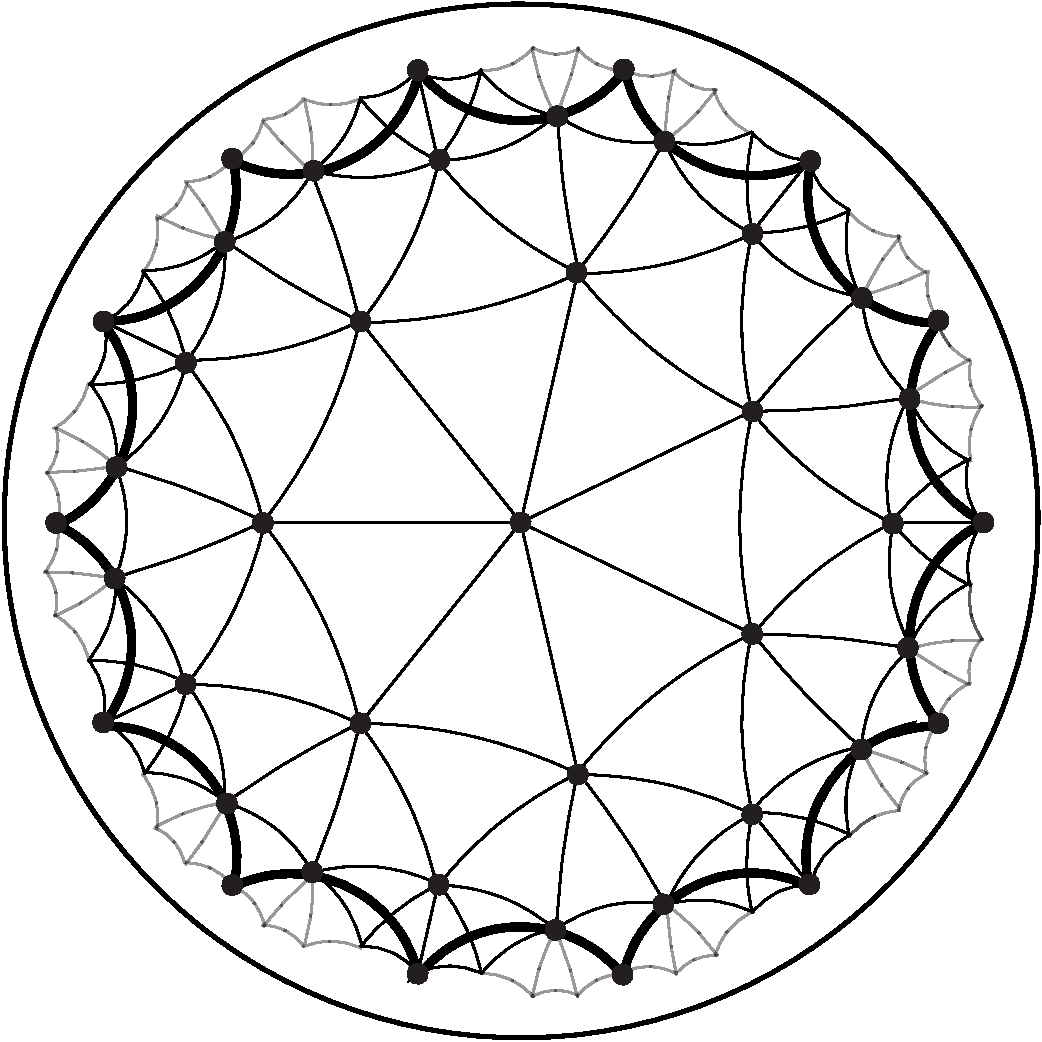
\includegraphics[width=2.75in]{figures/124_base}}}
    \qquad
    \subfloat[The refined tessellation $\Delta_T$]{{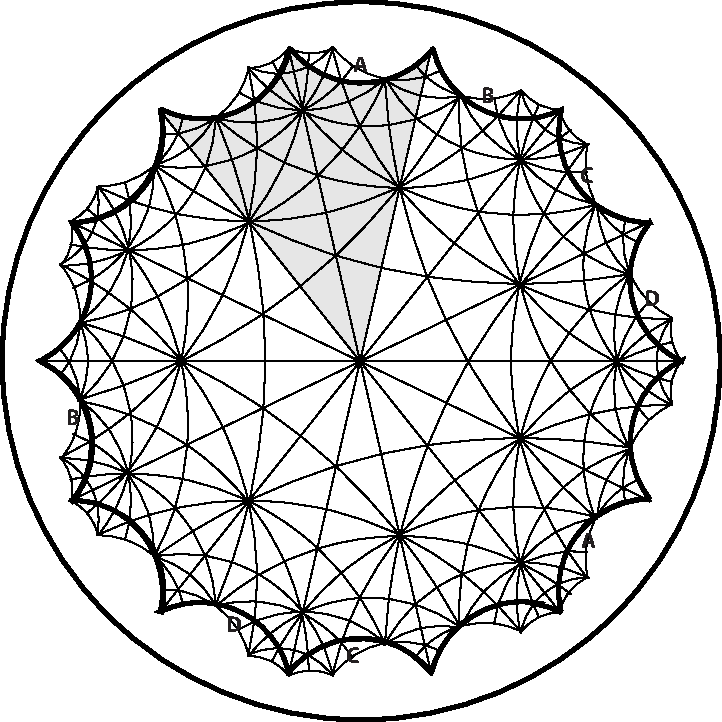
\includegraphics[width=2.75in]{figures/124_hyp}}}%
    \caption{Klein's quartic}%
    \label{fig:124}%
\end{figure}

A Weierstrass point on a non-singular irreducible algebraic curve $S$ is a point $P$ for which there exist functions on the curve with unusual pole orders at $P$ and no poles everywhere else. Hurwitz showed that if the genus $g$ is greater than 2, there there do exist Weierstrass points, and the number of Weierstrass points is bounded by $2g+2 \leq \omega \leq g(g+1)(g-1)$. Further, when genus $g \geq 2$, then $\Aut(S)$ is finite.  In characteristic zero, this can be proved by showing that every automorphism fixing more than $2g + 2$ points is the identity (by the Riemann-Roch theorem), and then obtaining a faithful representation of $\Aut(S)$ as permutations of the set of Weierstrass points $L: \text{Aut}(S) \to \Sigma_\omega$. Note that in general, the action of $\Aut(S)$ on the set of Weierstrass points is not transitive.

We calculate the Weierstrass points of a surface by finding the zeros of the Wronskian.
\begin{defn} Given a basis of holomorphic functions $\{f_1, \ldots , f_g\}$ on a Riemann surface $X$ of genus $g$, the Wronskian defined by $$\mathcal{W}(z) := \textrm{det} \left( \frac{d^j f_k(z)}{d z^j} \right)_{j = 0, \ldots , g - 1, \, k = 1, \ldots , g}$$ is a non-trivial holomorphic function on $X$ that induces a metric which we call the \textit{Wronski metric.} 
\end{defn}

\section{Verifications}

\label{verifications}

The results in Table \ref{table:plane} are proved as follows. The genus, their (non)-hyperelliptic nature, and their Weierstrass points are calculated by tools from section~\ref{sec:chap3}(??). The all-seeing tessellation $\Delta_T$ isconstructed using Section \ref{sec:allseeing}. 

We verify Conjecture ~\ref{tessconj} by using a seperate method of calculating automorphism groups. We derive the plane curve models of the cyclic covers of the sphere. With this input, calculate the automorphism group of the plane curve with: (1) our \texttt{autplane} program based on the algorithm in Jeroen-Sijsling-Zotine \cite{jeroen}, and (2) a group identification algorithm (written by the second author). The code used in this paper can all be found at \url{https://github.com/catherineray/aut-jac}.


\begin{table}[H]
\caption{Plane Curve Automorphism Groups}
\centering 
\begin{tabular}{ l | l c r r c} \hline
  \shortstack{Curve C} & Plane Curve Model & Genus & Aut(C) & $|$Aut(C)$|$ \\ \hline
   $\ast 8(1, 3, 4)$ & $y^2 - (x^5 - x)$ & 2 & $GL_2(F_3)$ & 48 \\ 
   $\ast 6(1, 1, 4)$  & $y^2 - (x^6 - 1)$ & 2 & $S_3 \rtimes D_4$  & 24 \\ 
  $7(1, 2, 4)$ (Klein's quartic) & $y^3x + x^3 + 1$ & 3 & $GL_3(F_2)$ & 168 \\  
  $8(1, 2, 5)$ (Fermat's quartic) & $y^4 - x (x+1) (x-1)$ & 3 & $C_4^{\text{ }2} \rtimes S_3$ & 96 \\
  $12(1, 3, 8)$ & $y^3 - (x^4 -1)$ & 3 & $C_4 \cdot A_4$ & 48 \\
   $\ast 8(1, 1, 6)$ & $y^2 - (x^8 - 1)$  & 3 &  $D_4 \rtimes C_4$ & 32 \\
  $\ast 12(1, 5, 6)$ &  $y^2 - (x^7 - x)$ & 3 & $C_4 \times S_3$ & 24 \\
  $\ast 4(1, 3, 3, 1)$ & $y^4 - (x^2-1) (x^2-a^2)^3$ & 3 & $C_2 \times D_8$ & 16 \\
  $5(1, 2, 4, 3)$ (Bring's curve) & $y^5 - x (x - 1)^2 (x + 1)^3$ & 4 & $S_5$ & 120 \\ 
  $12(1, 4, 7)$ (I-WP) & $y^3 - (x^5 - x)$ & 4 & $C_3 \times S_4$ & 72 \\ \hline 
\end{tabular}
\label{table:plane} 
\caption*{An $\ast$ indicates that the curve is hyperelliptic}
\end{table}

(for each example:)
-- plane curves
-- W points
-- hyperbolic tessellation
-- aut group


%In general, we find all-seeing tessellations on such surfaces $S$ using prior knowledge of the automorphism group of $S$. 

%the vertices are coming from the punctures in the underlying sphere, and the tesselation is a lift of the tesselation of the underling sphere (where we choose some special metric on the underlying sphere coming from Gauss Bonnet on the cyclic cover S?) 
%Is this correct?
%when you said "the special cases where we know the polyhedral tiling" do you mean we know those surfaces are quotients of polyhedral surfaces in R^3? 

%In some special cases, we know that our surface $S$ is in fact a quotient of a periodic polyhedral surface in $\R^3$, e.g. Fermat's curve, Schoen's I-WP Surface, and Bring's curve. In these very special cases, we can construct an all-seeing tessellation on $S$ without knowing the automorphism group of $S$ a priori. Thus, we can compute the automorphism group of $S$ from the all-seeing tessellation. \ti{prove that we can do it in the case of a quotient of a periodic polyhedral surface quotients?}

%\ti{Add some background here, define weierstrass points, mention Riemann roch, that it is a very rare property for the group to act transitively on the Weierstrass points, wronski to find them}
% Weierstrass points and Wronski are defined in section 2.1. Riemann-Roch is briefly mentioned there too.
\begin{thebibliography}{20}


\bibitem{jeroen}
N. Bruin, J. Sijsling, A. Zotine,
\textit{Numerical Computation of Endomorphism Rings of Jacobians},
\texttt{https://arxiv.org/pdf/1807.02605.pdf}

\bibitem{fk}
H. Farkas, I. Kra,
\textit{Riemann Surfaces},
Springer-Verlag, New York, 1992.

\bibitem{kw}
H. Karcher, M. Weber,
\textit{On Klein's Riemann Surface},
The Eightfold Way, MSRI Publications, 
Vol. 35, 1998, pp.9--49.

\bibitem{sl}
Z. Laing, D. Singerman,
\textit{Transitivity on Weierstrass Points}
Annales Academiae Scientiarum Fennicae Mathematica,
Vol. 37, 2012, pp.285--300

\bibitem{dami} 
D. Lee,
\textit{On a triply periodic polyhedral surface whose vertices are Weierstrass points},
Arnold Mathematical Journal, 
Vol. 3, Issue 3, 2017, pp.319--331.

\bibitem{dthesis} 
D. Lee, 
\textit{Geometric realizations of cyclically branched coverings over punctured spheres},
\texttt{https://arxiv.org/abs/1809.06321}, preprint.

\bibitem{hyp}
R. Lercier, C. Ritzenthaler, J. Sijsling,
\textit{Fast computation of isomorphisms of hyperelliptic curves and explicit Galois descent},
Proceedings of the Tenth Algorithmic Number Theory Symposium, 2013, pp. 463–-486.

\bibitem{matti} 
M. Weber,
\textit{Kepler's small stellated dodecahedron as a Riemann surface},
Pacific Journal of Mathematics, 
Vol. 220, 2005, pp.167--182.

\end{thebibliography}

\end{document}